\section{CANae}
\subsection{Introducción}
\begin{frame}
	\frametitle{CANae}
	\begin{itemize}
		\item Surge de la necesidad de desarrollar un protocolo:
		\begin{itemize}
			\item Que actúe en las capas superiores del modelo de OSI
			\item Basado en el protocolo CAN
			\item Que permita la distribución de las tareas y el procesamiento llevado a cabo por los nodos
		\end{itemize}
		\item CANae se divide la capa de aplicaciones en dos:
		\begin{itemize}
			\item CANae Application Layer
			\item CANae High Application Layer
		\end{itemize}
	\end{itemize}
\end{frame}

\subsection{Capa de aplicación}
\begin{frame}
	\frametitle{Capa de Aplicación}
	\centering
	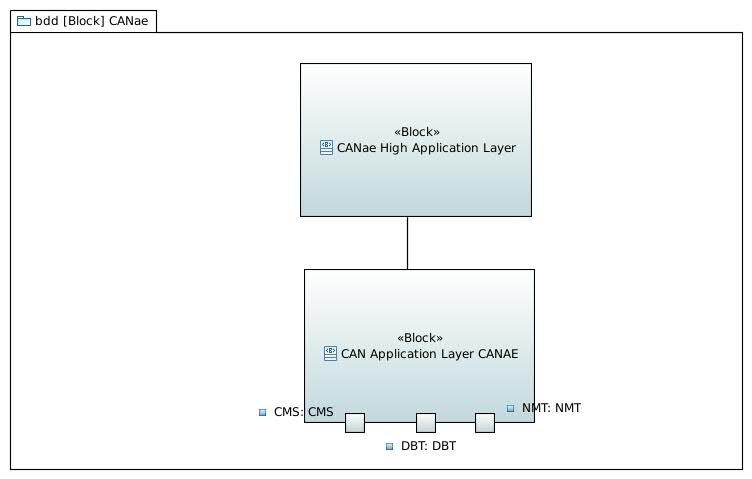
\includegraphics[scale=0.4]{images/CANAE.JPG}
\end{frame}

\subsection{CANae Application Layer}
\begin{frame}
	\frametitle{Capa de Aplicación}
	\centering
	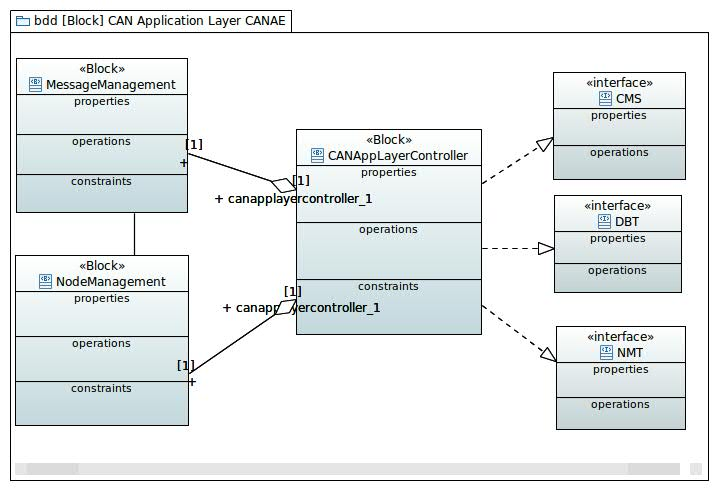
\includegraphics[scale=0.4]{images/CAN_Application_Layer_CANAE.jpg}
\end{frame}

% \subsection{CMS}
\begin{frame}
	\frametitle{CAN bassed Message Specification (CMS)}
	\centering
	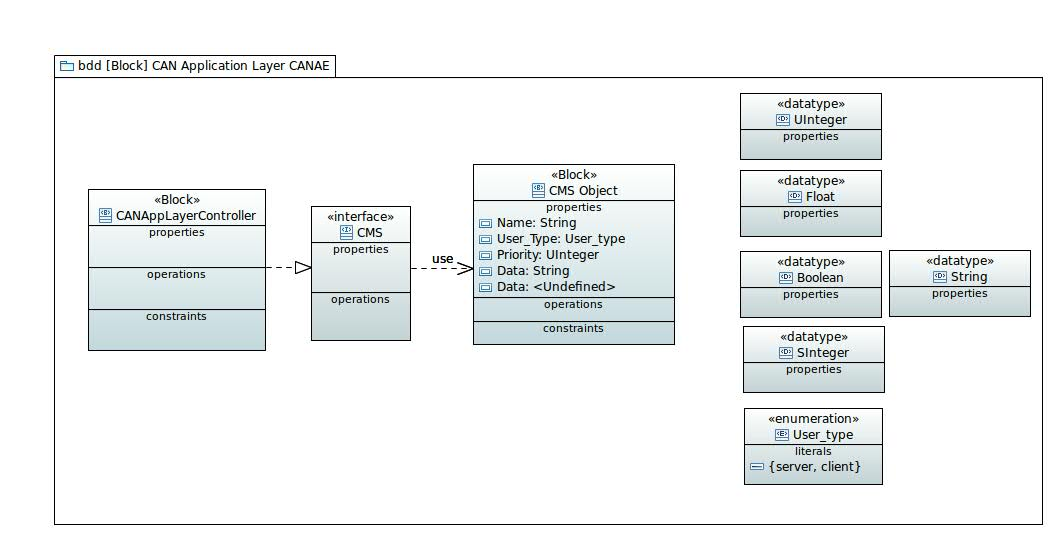
\includegraphics[scale=0.3]{images/CMS.JPG}
\end{frame}

% \subsection{NMT}
\begin{frame}
	\frametitle{Network Management (NMT)}
	\centering
	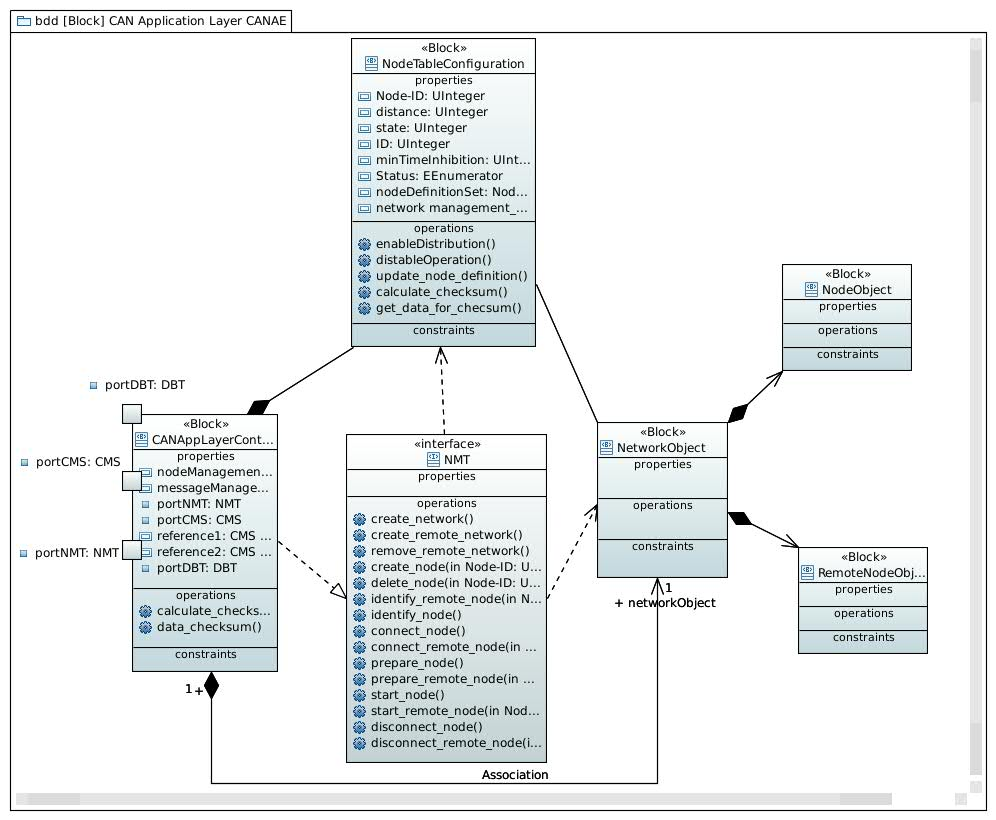
\includegraphics[scale=0.25]{images/NMT.JPG}
\end{frame}

% \subsection{DBT}
\begin{frame}
	\frametitle{Distributor (DBT)}
	\centering
	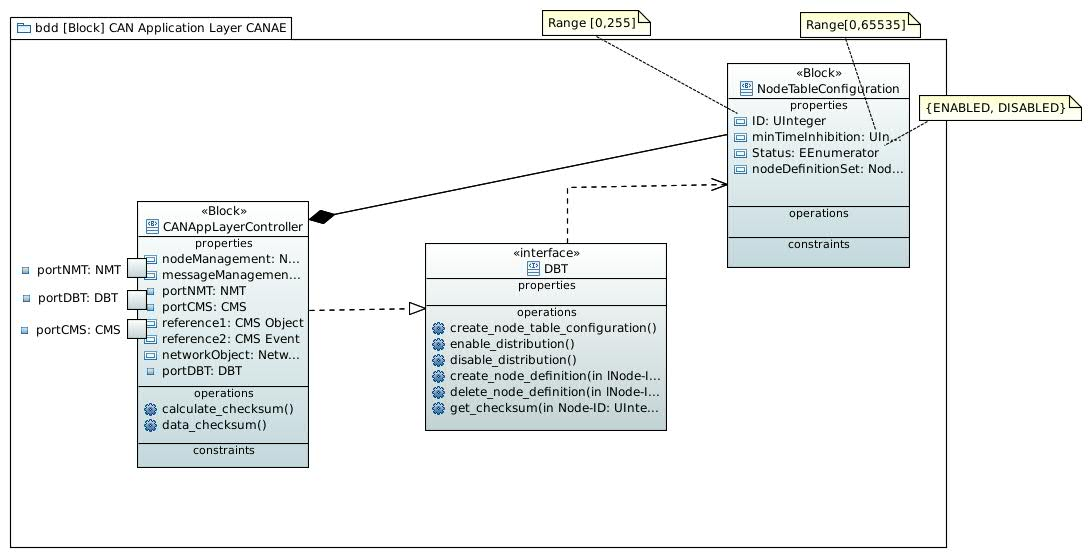
\includegraphics[scale=0.3]{images/DBT.JPG}
\end{frame}

% \subsection{Formato de mensaje}
\begin{frame}
	\frametitle{Formato del mensaje}
	\centering
	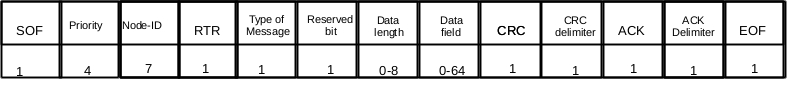
\includegraphics[scale=0.4]{images/Data_Frame.jpg}
\end{frame}

\subsection{High Application Layer CANae}
\begin{frame}
	\frametitle{High Application Layer CANae}
	\centering
	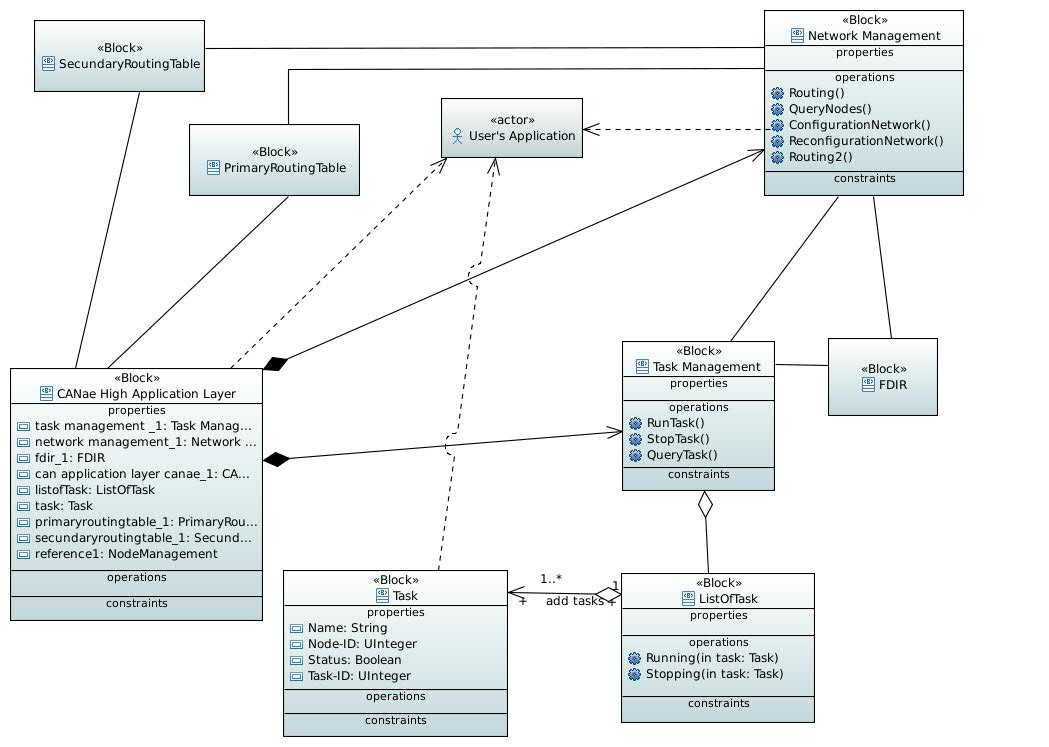
\includegraphics[scale=0.3]{images/CANae_High_App_Layer.JPG}
\end{frame}